%%%%%%%%%%%%%%%%%%%%%%%%%%%%%%%%%%%%%%%%%
% Stylish Article
% LaTeX Template
% Version 2.1 (1/10/15)
%
% This template has been downloaded from:
% http://www.LaTeXTemplates.com
%
% Original author:
% Mathias Legrand (legrand.mathias@gmail.com) 
% With extensive modifications by:
% Vel (vel@latextemplates.com)
%
% License:
% CC BY-NC-SA 3.0 (http://creativecommons.org/licenses/by-nc-sa/3.0/)
%
%%%%%%%%%%%%%%%%%%%%%%%%%%%%%%%%%%%%%%%%%

%----------------------------------------------------------------------------------------
%	PACKAGES AND OTHER DOCUMENT CONFIGURATIONS
%----------------------------------------------------------------------------------------

\documentclass[fleqn,10pt]{SelfArx} % Document font size and equations flushed left

\usepackage{subcaption}
\usepackage[english]{babel} % Specify a different language here - english by default
\usepackage{array,booktabs}% http://ctan.org/pkg/{array,booktabs}
\usepackage{lipsum} % Required to insert dummy text. To be removed otherwise
\usepackage[section]{placeins}

\newcolumntype{P}[1]{>{\centering\arraybackslash}p{#1}}
\newcolumntype{M}[1]{>{\centering\arraybackslash}m{#1}}
%----------------------------------------------------------------------------------------
%	COLUMNS
%----------------------------------------------------------------------------------------

\setlength{\columnsep}{0.55cm} % Distance between the two columns of text
\setlength{\fboxrule}{0.75pt} % Width of the border around the abstract

%----------------------------------------------------------------------------------------
%	COLORS
%----------------------------------------------------------------------------------------

\definecolor{color1}{RGB}{0,0,90} % Color of the article title and sections
\definecolor{color2}{RGB}{0,20,20} % Color of the boxes behind the abstract and headings

%----------------------------------------------------------------------------------------
%	HYPERLINKS
%----------------------------------------------------------------------------------------

\usepackage{hyperref} % Required for hyperlinks
\hypersetup{hidelinks,colorlinks,breaklinks=true,urlcolor=color2,citecolor=color1,linkcolor=color1,bookmarksopen=false,pdftitle={Title},pdfauthor={Author}}

%----------------------------------------------------------------------------------------
%	ARTICLE INFORMATION
%----------------------------------------------------------------------------------------

\JournalInfo{01/28/2016} % Journal information
\Archive{} % Additional notes (e.g. copyright, DOI, review/research article)

\PaperTitle{ESE650 Project 1: Color Segmentation} % Article title

\Authors{Nischal K N\\nischal@seas.upenn.edu} % Authors
%\affiliation{\textsuperscript{1}\textit{Department of Biology, University of Examples, London, United Kingdom}} % Author affiliation
%\affiliation{\textsuperscript{2}\textit{Department of Chemistry, University of Examples, London, United Kingdom}} % Author affiliation
%\affiliation{*\textbf{Corresponding author}: john@smith.com} % Corresponding author

\Keywords{} % Keywords - if you don't want any simply remove all the text between the curly brackets
\newcommand{\keywordname}{Keywords} % Defines the keywords heading name

%----------------------------------------------------------------------------------------
%	ABSTRACT
%----------------------------------------------------------------------------------------

\Abstract{Detection of unique objects such as cones, barrels, signs, etc is a crucial part of robotic system be it autonomous cars or humanoids. In this project an approach to detect barrels based on their color and physical dimensions has been discussed. Gaussian mixture models(GMM) are used to model the color of the barrel including variations at different lighting conditions and is used to perform color segmentation. A series of morphological operations and filtering based on dimensions of the segments are performed to determine the barrel and overcome occlusion. The model is created from a training set and evaluated on a separate test set. The performance of the test set is shown in this report.}

%----------------------------------------------------------------------------------------

\begin{document}

\flushbottom % Makes all text pages the same height

\maketitle % Print the title and abstract box

\tableofcontents % Print the contents section

\thispagestyle{empty} % Removes page numbering from the first page

%----------------------------------------------------------------------------------------
%	ARTICLE CONTENTS
%----------------------------------------------------------------------------------------

\section{Introduction} % The \section*{} command stops section numbering

%\addcontentsline{toc}{section}{Introduction} % Adds this section to the table of contents

In this project red colored barrels are detected from static high resolution images by color segmentation using Gaussian mixture model(GMM). First the model of the red colored pixels is generated using a multi-variance GMM on a custom color space designed to highlight the red regions of the barrel. To cluster the pixels into gaussians, EM optimization is used. Additionally the parameters such as height,width and distance from camera of the barrel on the training set is recorded and modeled.

To detect the barrels in a given image, the probability of each pixel belonging to a Gaussian is determined. A likelihood map of all the pixels is generated. From this a binary image is created by thresholding the probabilities. A series of morphological operations are performed to remove noise and small stray clusters. Finally from the model of heights and widths of barrel generated during training, the barrel is detected and its distance is estimated.

%------------------------------------------------

\section{Methods}
The process was divided into 2 parts, viz., training which was performed offline to generate the model and then this model was used on testing images to determine the centers and distances of the barrel from the camera. The block diagram of the entire process is shown in Fig. \ref{fig:block}.

\begin{figure}[hbtp]
\centering
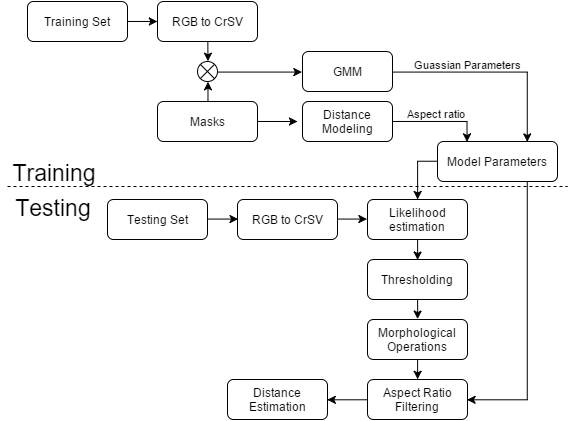
\includegraphics[scale=0.45]{block.png}
\caption{Block diagram}
\label{fig:block}
\end{figure}

The training process involved generation of masks to separate the barrel pixels form rest of the image for modeling. This was done using roipoly function in matlab.

\subsection{Color Space}
Choosing a particular color space was extremely important because of wide variation in the illumination of the barrels from outdoors to indoors to dark rooms. Choosing a right color space makes the system robust to illumination changes. 

\begin{figure}[hbtp]
\centering
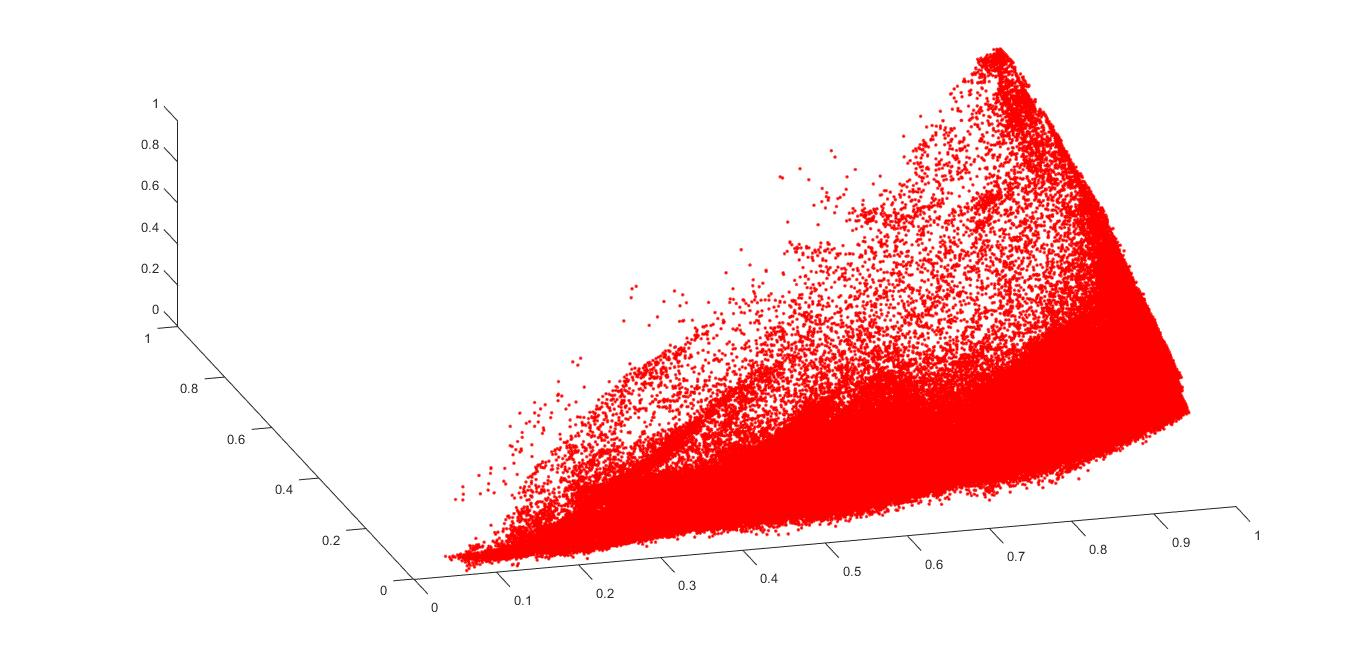
\includegraphics[scale=0.15]{RGB.jpg}
\caption{Scatter plot for RGB color space}
\label{fig:rgb}
\end{figure}

First RGB color space was evaluated. The scatter plot of the red pixels spread over half the entire space making it less unique(Fig. \ref{fig:rgb}). HSV color space however performed better for illumination variations, but also had quite a few outliers. Similarly YCbCr was not robust enough. This can be seen from the scatter plots in Fig. \ref{fig:hsv} and Fig. \ref{fig:ycbcr}.

\begin{figure}[hbtp]
\centering
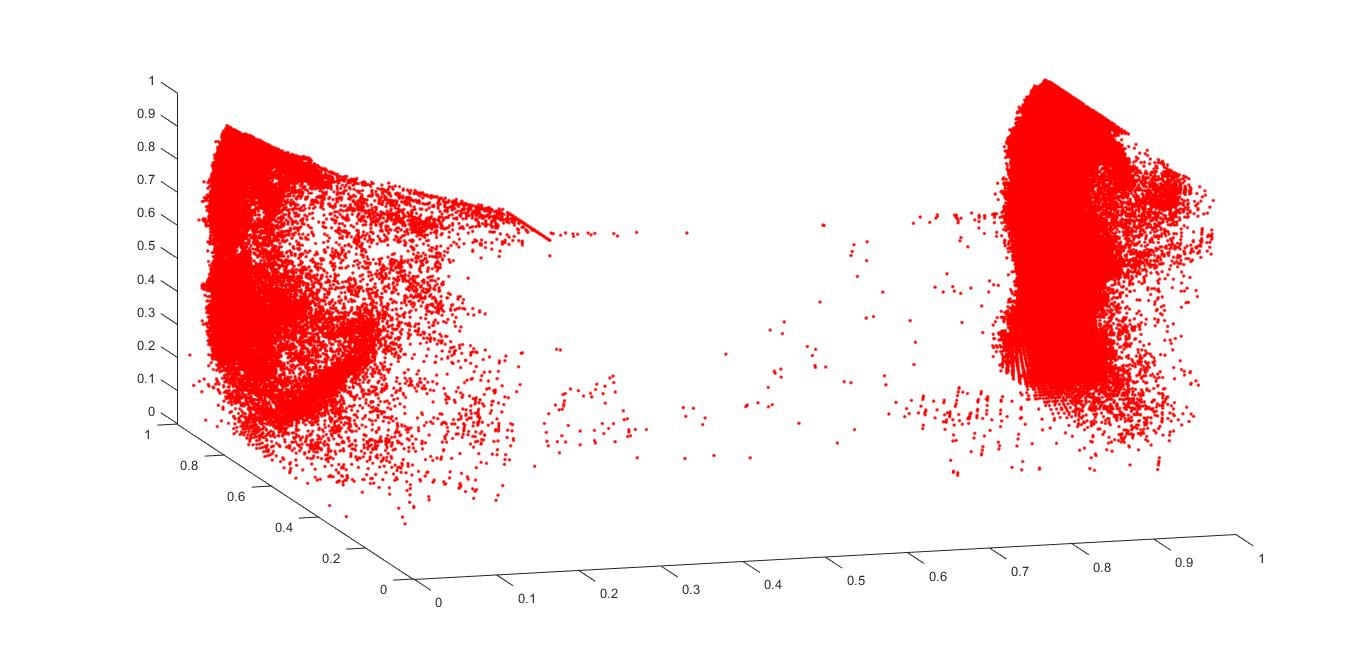
\includegraphics[scale=0.15]{hsv.jpg}
\caption{Scatter plot for HSVB color space}
\label{fig:hsv}
\end{figure}

\begin{figure}[hbtp]
\centering
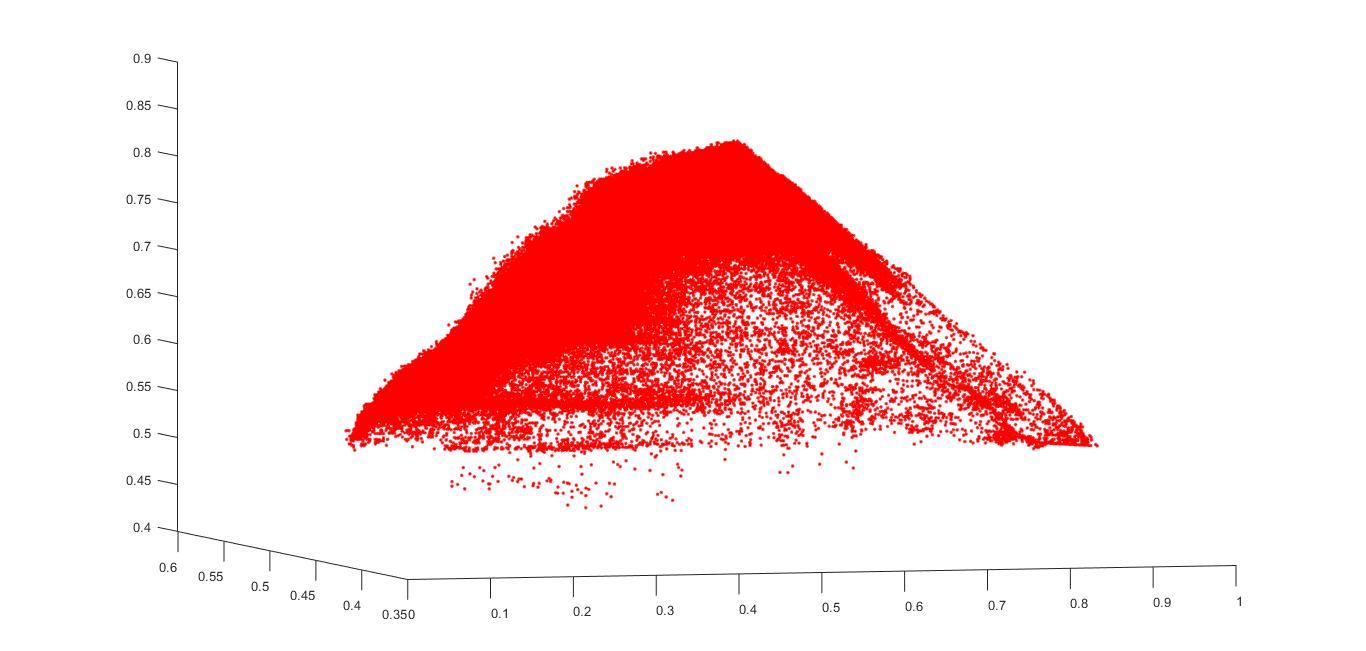
\includegraphics[scale=0.15]{ycbcr.jpg}
\caption{Scatter plot for YCbCr color space}
\label{fig:ycbcr}
\end{figure}

\begin{figure}[hbtp]
\centering
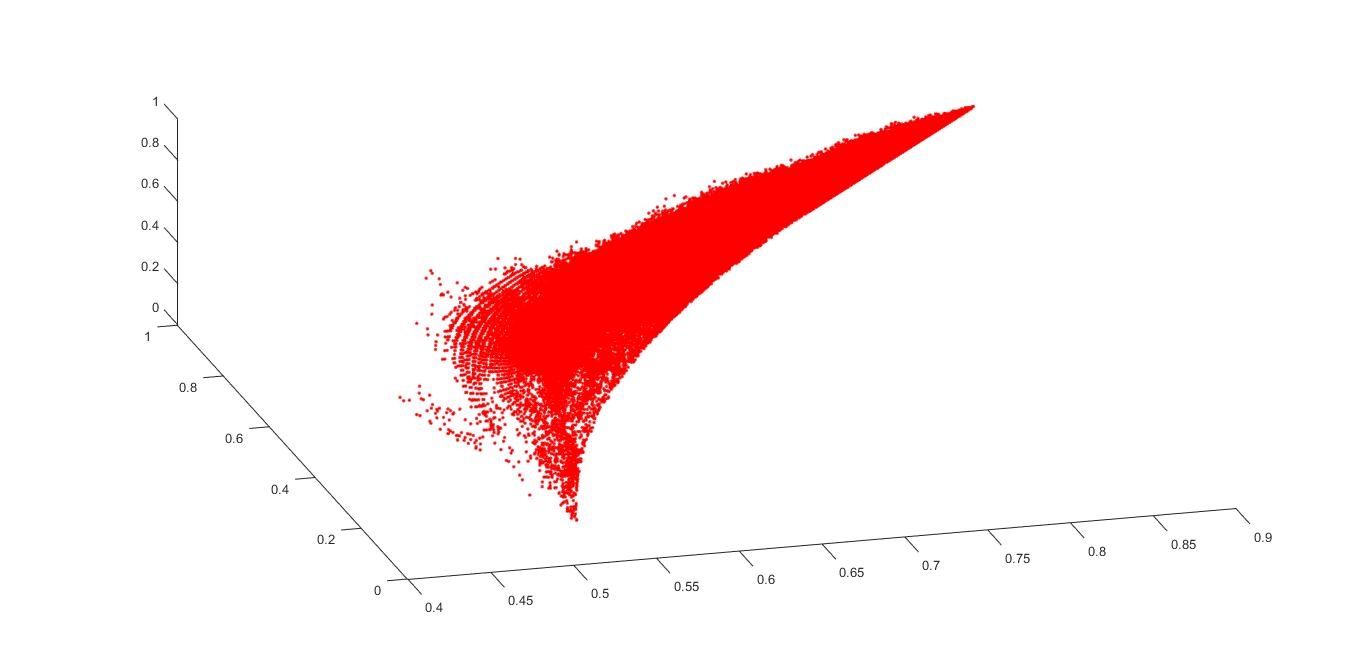
\includegraphics[scale=0.15]{custom.jpg}
\caption{Scatter plot of CrSV color space}
\label{fig:CrSV}
\end{figure}

Finally a custom color space using S and V components of HSV and Cr component of YCbCr helped to capture the variations perfectly. It can be seen from the scatter plot(Fig. \ref{fig:CrSV})  that all the pixels are bunched much closely together and also there are no outliers. This allows easy classification of red pixels from others.

\begin{figure*}[htb!]
\centering
\begin{minipage}[b]{.24\textwidth}
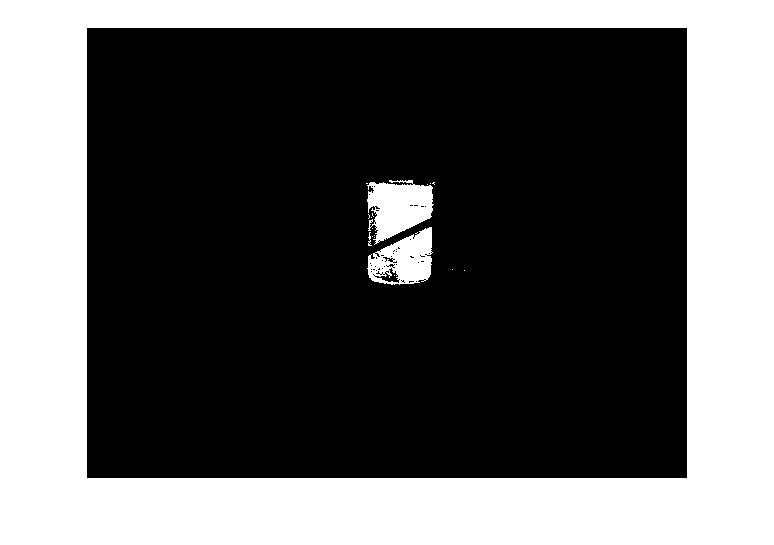
\includegraphics[trim={3cm 2cm 3cm 2cm},clip,scale=0.19]{mp1.jpg}
\subcaption{Segmented Image}\label{label-a}
\end{minipage}
\begin{minipage}[b]{.24\textwidth}
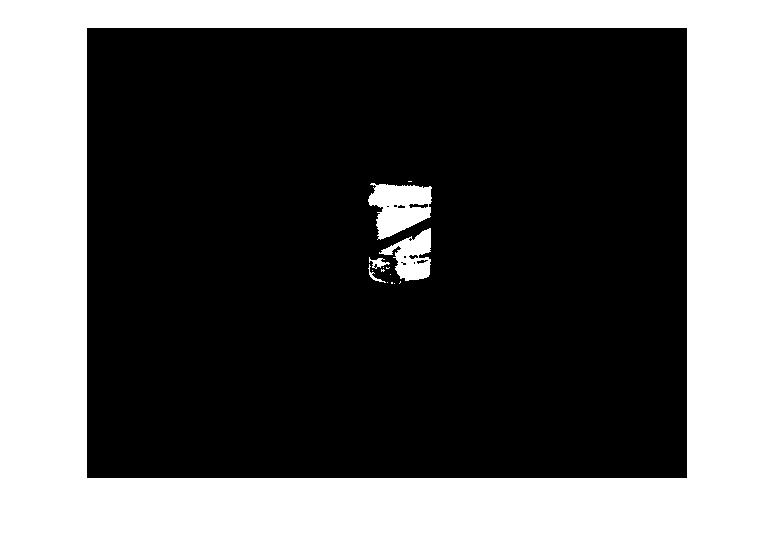
\includegraphics[trim={3cm 2cm 3cm 2cm},clip,scale=0.19]{mp2.jpg}
\subcaption{erode 1}\label{label-b}
\end{minipage}
\begin{minipage}[b]{.24\textwidth}
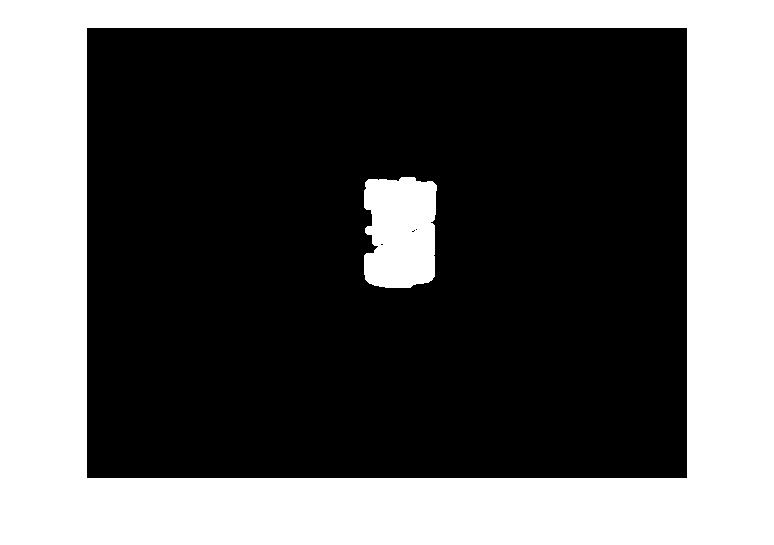
\includegraphics[trim={3cm 2cm 3cm 2cm},clip,scale=0.19]{mp3.jpg}
\subcaption{dilate}\label{label-b}
\end{minipage}
\begin{minipage}[b]{.24\textwidth}
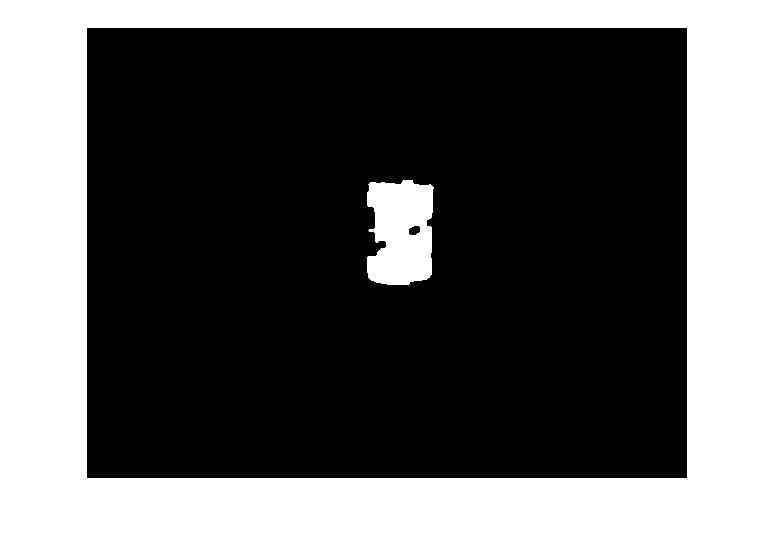
\includegraphics[trim={3cm 2cm 3cm 2cm},clip,scale=0.19]{mp4.jpg}
\subcaption{erode 2}\label{label-b}
\end{minipage}
\caption{Morphological operations to join blobs}
\label{fig:morph}
\end{figure*}

\subsection{Gaussian Mixture Model}
Initially a single Gaussian was used to model the color space. As the distribution was not truly ellipsoidal, the entire information was not captured well. Hence detection of few shades of red was unsuccessful as shown in Fig. \ref{fig:sg} which is the segmented image of Fig. \ref{fig:sg_org}. 

\begin{figure}[t]
\centering
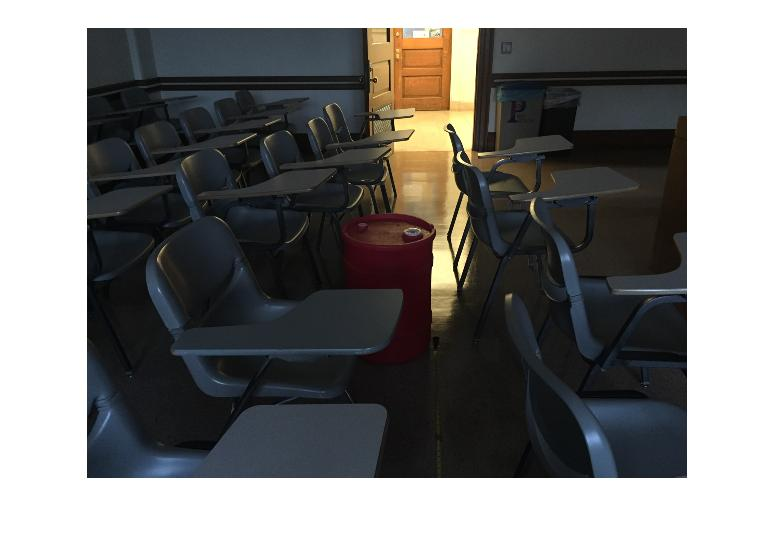
\includegraphics[scale=0.2]{sg_org.jpg}
\caption{An image at which a single Gaussian fails}
\label{fig:sg_org}
\end{figure}
\begin{figure}[t]
\centering
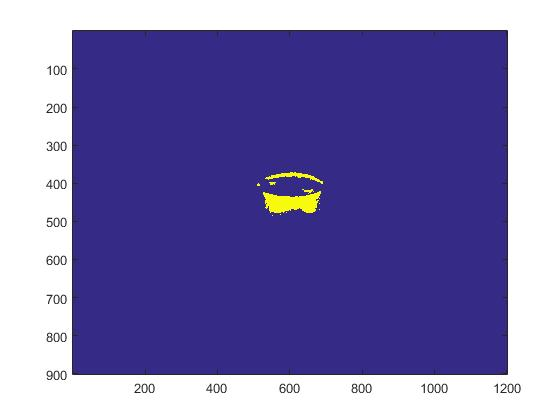
\includegraphics[scale=0.3]{sg.jpg}
\caption{Segmented image at which a single Gaussian fails}
\label{fig:sg}
\end{figure}

\begin{figure}[t]
\centering
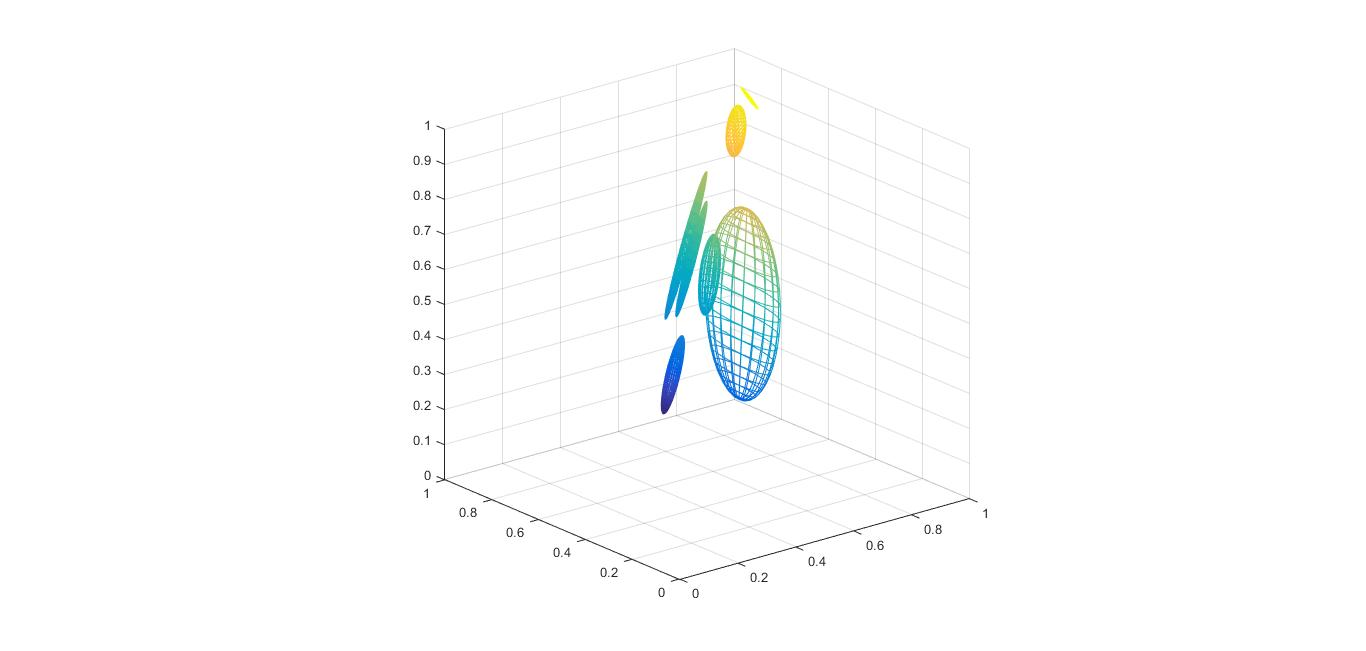
\includegraphics[trim={11cm 2cm 3cm 2cm},clip,scale=0.3]{elip.jpg}
\caption{Ellipsoidals representing guassians of CrSV}
\label{fig:ellip}
\end{figure}

The parametric model using a single Gaussian for a pixel X was modeled as in equation.

\[
P(X\mid Color) = \frac{1}{\sqrt{(2\pi)^3det(A)}}\exp \left(\frac{(X - \mu)^\top A^{-1} (X - \mu)}{-2} \right)
\]

where, A is the co-variance matrix and $\mu$ is the mean of the Gaussian distribution.


The performance of the system was drastically improved by using a mixture of such Gaussians with variable variance. Expectation Maximization algorithm was used to optimize the distribution parameters. The mean, variance and weights of each cluster was generated randomly and then the EM algorithm determined the optimal parameters. Cross validation was performed to determine the number of clusters by comparing the masks generated with the hand labeled masks. Fig. \ref{fig:ellip} shows the region of the color space modeled by GMM. It can be seen that the area of the scatter plot modeled is much greater than a single Gaussian. As a result the likelihood model captures the barrel pixels much better than single Gaussian.

\subsection{Morphological operations}

The training set consists of images with barrels that are occluded by poles and railings. One way of handling this was by using morphological operations such as erode and dilate. The following sequence of operations was performed and the corresponding outputs are shown in Fig. \ref{fig:morph}.
\begin{enumerate}
\item Erode operation with a disk structural element of size 1 which removes all the stray pixels.
\item Dilate operation with a disk structural element of size 10 which bridges the gaps between disconnected components of the barrel.
\item Second Erode operation with a disk structural element of size 7 to prevent the barrel blowing up in size which can affect the distance estimate.
\end{enumerate}

\subsection{Aspect Ratio filtering}
After the series of morphological operations, blobs are detected on the resulting image using regionprops. The series of blobs detected are filtered through aspect ratio check which was modeled during training. During training, the ratio of height to width for all the hand labeled masks was calculated. The mean aspect ratio and the standard deviation was used as the parameters to filter the blobs. The threshold was set to 3 times the standard deviation. 

\begin{figure}[h]
\centering
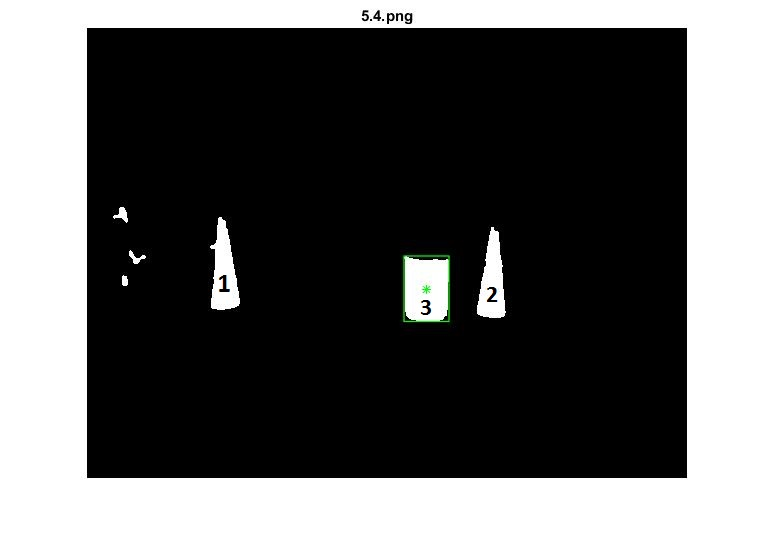
\includegraphics[trim={2cm 2cm 3cm 2cm},clip,scale=0.4]{ar.jpg}
\caption{Rejection of blobs based on aspect ratio}
\label{fig:ar}
\end{figure}

\[ meanAR-3*sdAR < AspectRatio < meanAR+3*sdAR
\]
where meanAR is the mean aspect ration and sdAR is the standard deviation of aspect ratio obtained from training.
The major and minor axis length of each blob was determined form regionprops and its aspect ratio was calculated. The blob was retained if the aspect ratio matched the above criteria, else was eliminated. It can be seen from Fig. \ref{fig:ar}, blobs 1 and 2 do not match the aspect ratio and are eliminated. But however this also led to failure in detection of occluded barrels in the test set shown in Table \ref{tab:results}, Image 003.png.


\subsection{Center and Distance Estimation}
Once the barrel was detected based on the aspect ratio the center of mass of the blob was determined using regionprops. The distance of the barrel was estimated using the width of the barrel which was again obtained from the minor axis of regionprops. From the training set, it was seen that the width of the barrel was proportional to inverse of distance. Thus a linear regression model was fit into this data to obtain the coefficients(Fig. \ref{fig:dist_graph}).
\begin{align*}
width \propto \frac{1}{distance}
\end{align*}

\begin{figure}[ht]
\centering
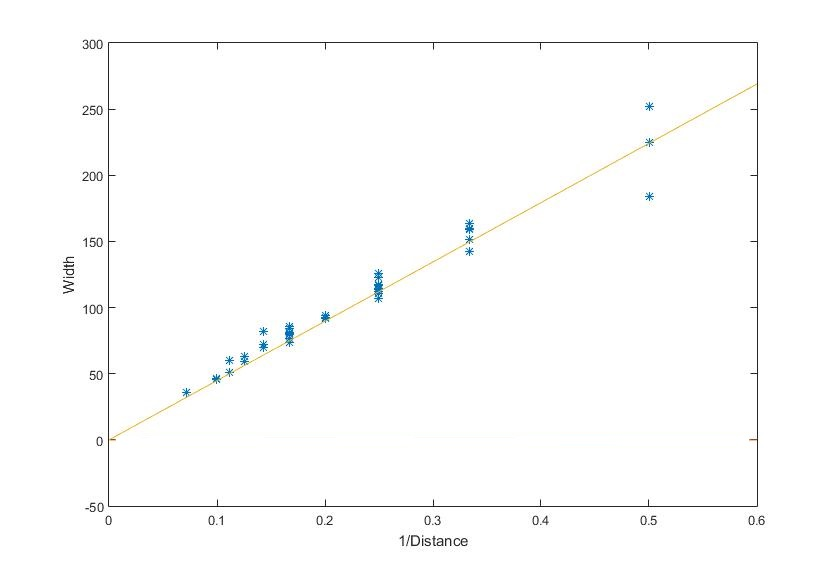
\includegraphics[scale=0.35]{graph2.jpg}
\caption{Variation of distance wrt width}
\label{fig:dist_graph}
\end{figure}

\section{Results}
The above algorithm was run on 10 test images. The centers and the distances are tabulated in Table \ref{tab:results}. The segmented images are shown in the same table with the center marked with a red *. The green star on the original image also shows the center. The parameters of the model used in evaluation are listed in Table \ref{tab:parameters}. From the results, it can be seen that improper erosion and dilation affected a few results. 

\begin{table}[t]
\caption{Parameters of the model}
\centering
\begin{tabular}{cc}
\toprule
Parameter & Value \\ 
\midrule
Clusters & 7 \\ 
Mean Aspect Ratio & 1.5371 \\ 
SD of Aspect Ratio & 0.102 \\ 
Aspect Ration thershold & 3 \\ 
Distance Model & $0.0022\times w-0.0096$ \\ 
\bottomrule
\end{tabular} 
\label{tab:parameters}
\end{table}

\section{Discussion and Conclusion}
The incorrect result of 002.png can be traced to incorrect erosion and dilation process. 002.png failed due to minimal dilation preventing the two parts of the barrel to merge. But however this prevented merging of 2 the barrels in image 003.png. Hence one of the barrel was rightly detected while the other barrel even though segmented properly was rejected due to incorrect aspect ratio. More than half the barrel was hidden which drastically changed the aspect ratio. 

Image 008.jpg was detected successfully as 3/4th of the barrel was visible in the bottom portion, but however the distance estimate was way off due to incorrect width measurement. This can be compensated by using both the height and the width of the barrel along with the detected area to determine the distance over just using width. 
Image 007.png and 005.png were captured pretty well because of the new color space that normalized most of the lighting effect.

The drawback of the current process is that the blobs are filtered based on only aspect ratio. This fails when the object is occluded as seen in some of the test sets. 

\begin{table*}
\caption{Results on test images}
\centering
\begin{tabular}{>{\centering\arraybackslash}M{15mm}cc>{\centering\arraybackslash}M{11mm}>{\centering\arraybackslash}M{15mm}}
\hline 
Image No & Original Image & Segmented image & Center & Distance \\ 
\hline 
\vspace{-4cm}001.png & 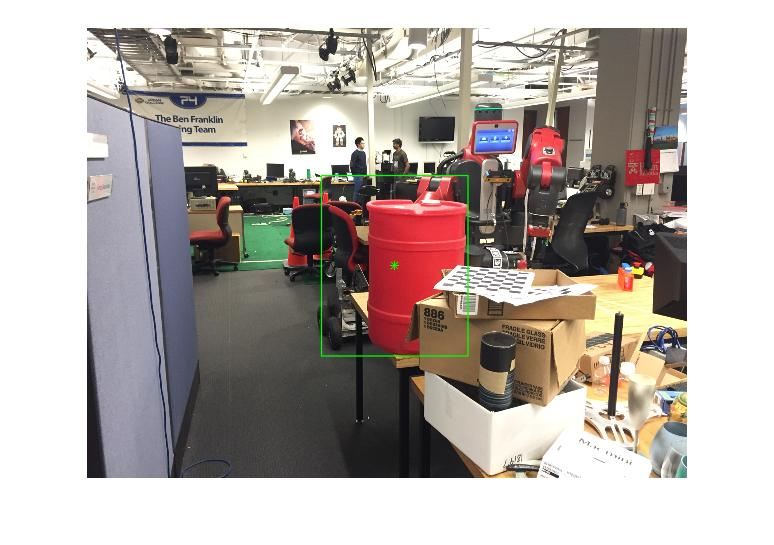
\includegraphics[trim={3cm 2cm 3cm 2cm},clip,scale=0.28]{results/001.jpg} & 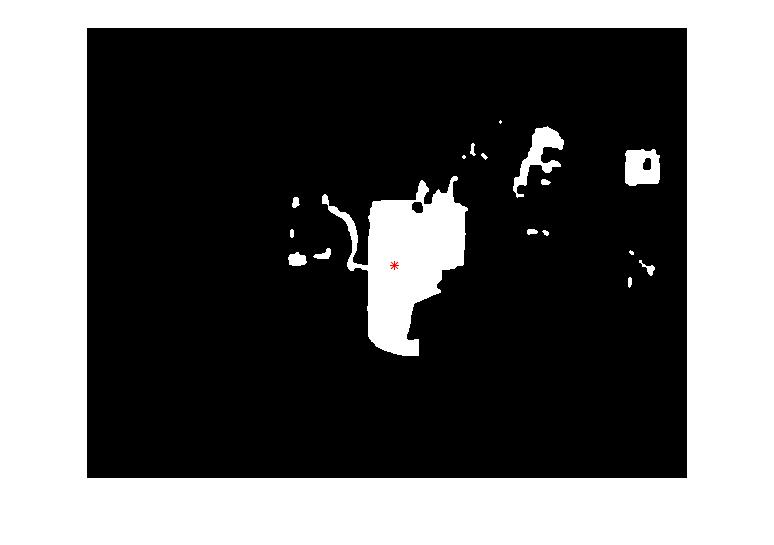
\includegraphics[trim={3cm 2cm 3cm 2cm},clip,scale=0.28]{results/001s.jpg} & \vspace{-4cm} x = 616, y = 476 & \vspace{-4cm}2.0969 \\ 
\hline 
\vspace{-4cm}002.png & 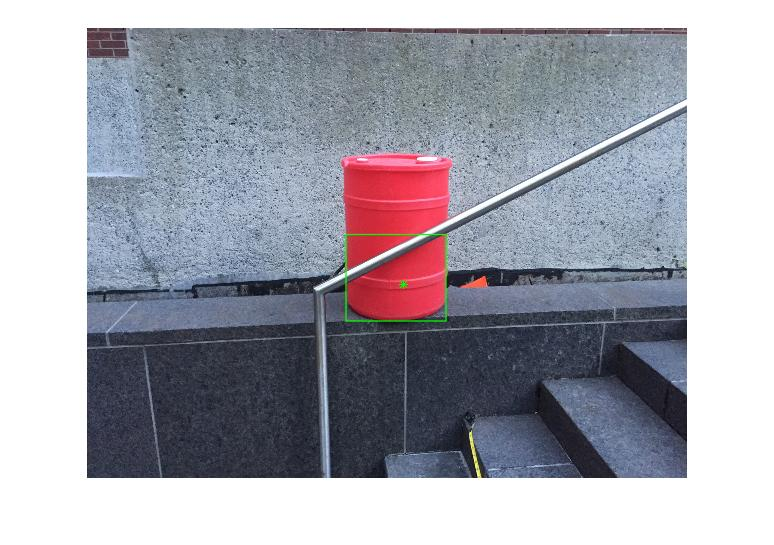
\includegraphics[trim={3cm 2cm 3cm 2cm},clip,scale=0.28]{results/002.jpg} & 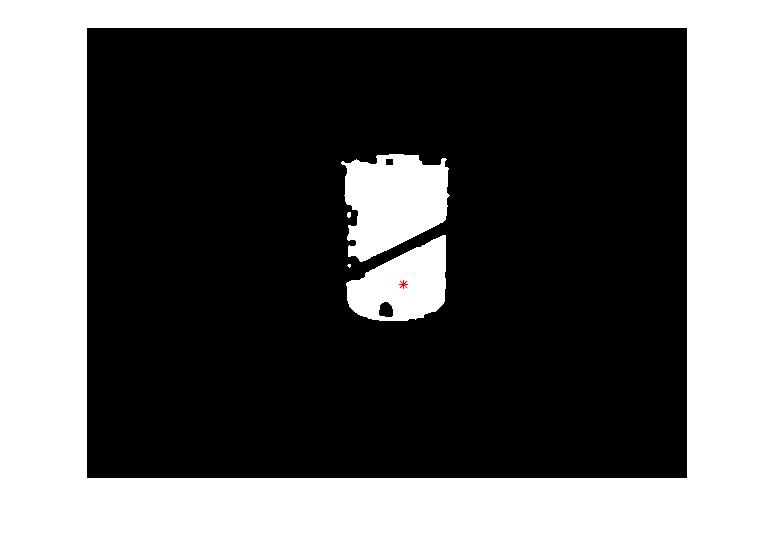
\includegraphics[trim={3cm 2cm 3cm 2cm},clip,scale=0.28]{results/002s.jpg} & \vspace{-4cm} x = 633.13, y = 513.52 & \vspace{-4cm}3.3666 \\ 
\hline 
\vspace{-4cm}003.png & 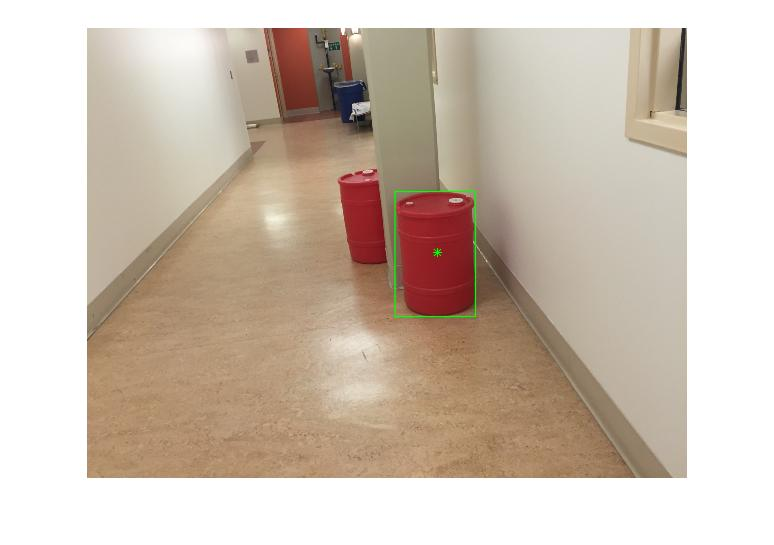
\includegraphics[trim={3cm 2cm 3cm 2cm},clip,scale=0.28]{results/003.jpg} & 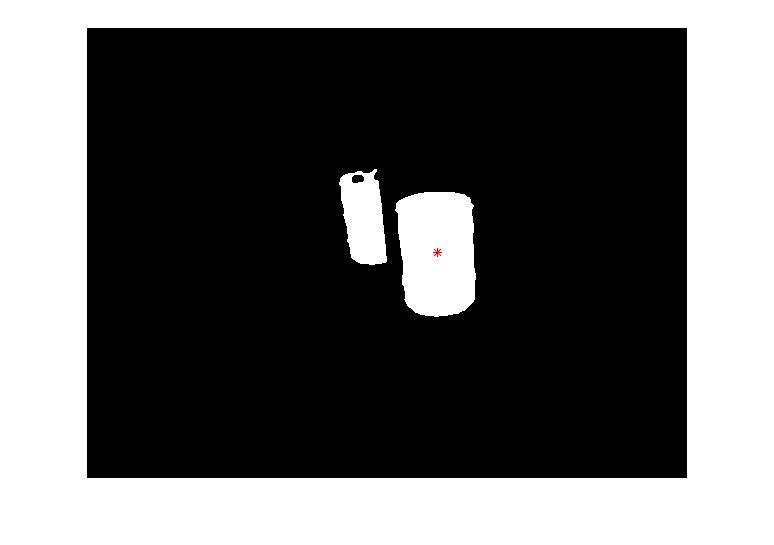
\includegraphics[trim={3cm 2cm 3cm 2cm},clip,scale=0.28]{results/003s.jpg} & \vspace{-4cm} x = 700.65, y = 448.93 & \vspace{-4cm}2.7914 \\ 
\hline 
\vspace{-4cm}004.png & 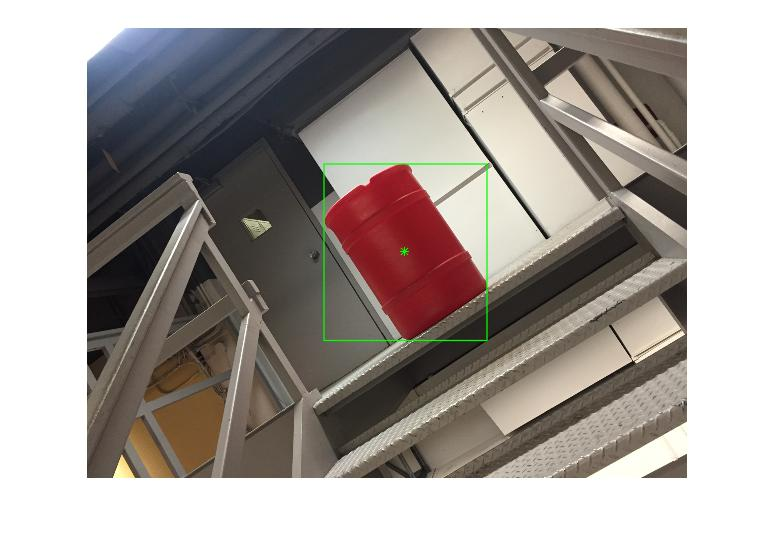
\includegraphics[trim={3cm 2cm 3cm 2cm},clip,scale=0.28]{results/004.jpg} & 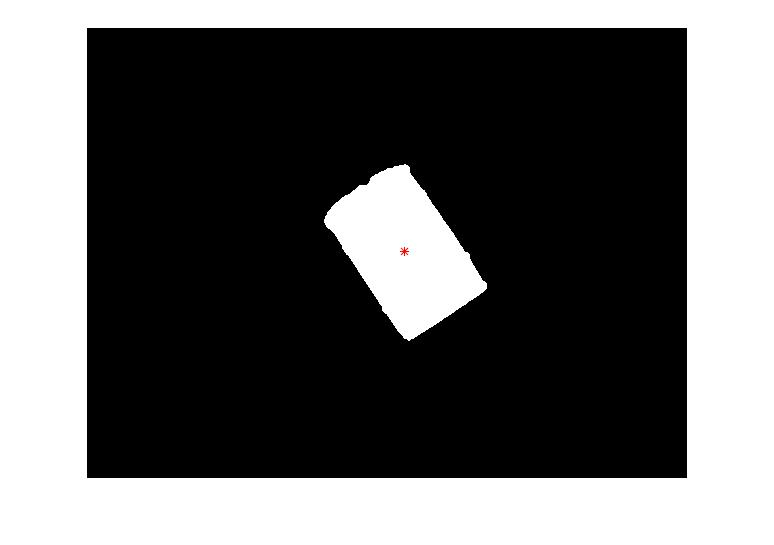
\includegraphics[trim={3cm 2cm 3cm 2cm},clip,scale=0.28]{results/004s.jpg} & \vspace{-4cm} x = 635.52, y = 446.75 & \vspace{-4cm}1.9983 \\ 
\hline 
\vspace{-4cm}005.png & 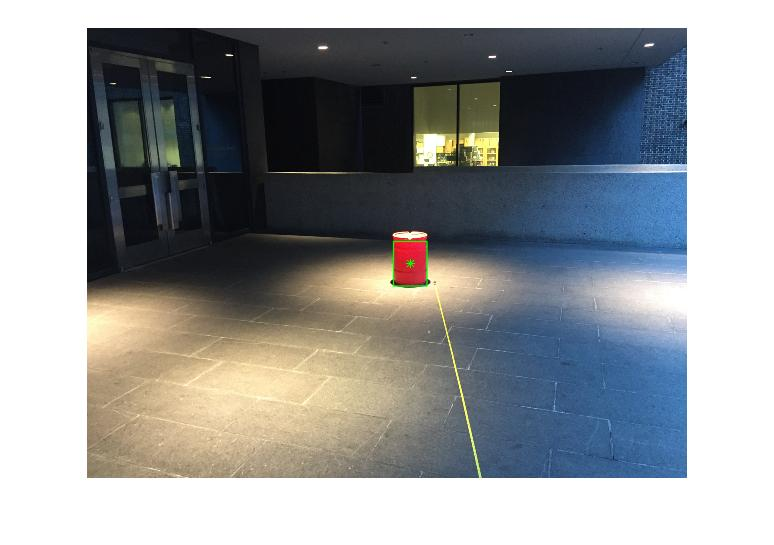
\includegraphics[trim={3cm 2cm 3cm 2cm},clip,scale=0.28]{results/005.jpg} & 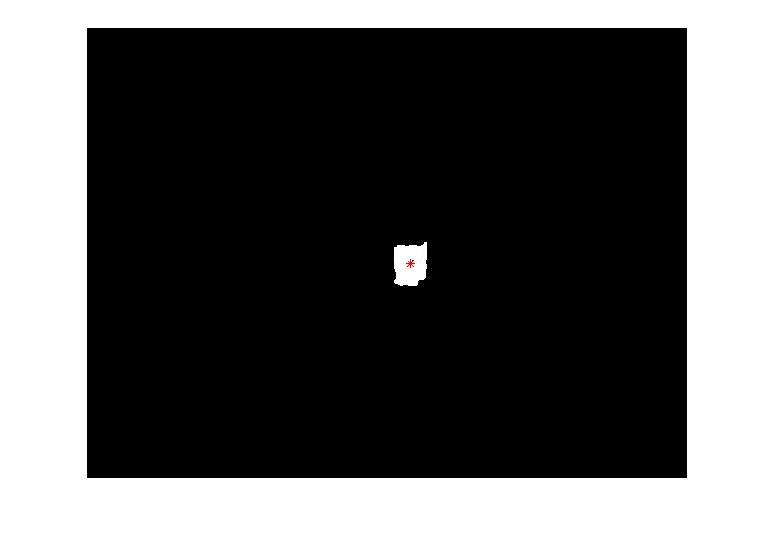
\includegraphics[trim={3cm 2cm 3cm 2cm},clip,scale=0.41]{results/005s.jpg} & \vspace{-4cm} x = 647, y = 472 & \vspace{-4cm}8.1899 \\ 
\hline 
\end{tabular} 
\label{tab:results}
\end{table*}

\begin{table*}
\centering
\begin{tabular}{>{\centering\arraybackslash}M{15mm}cc>{\centering\arraybackslash}M{11mm}>{\centering\arraybackslash}M{15mm}}
\hline 
Image No & Original Image & Segmented image & Center & Distance \\ 
\hline 
\vspace{-4cm}006.png & 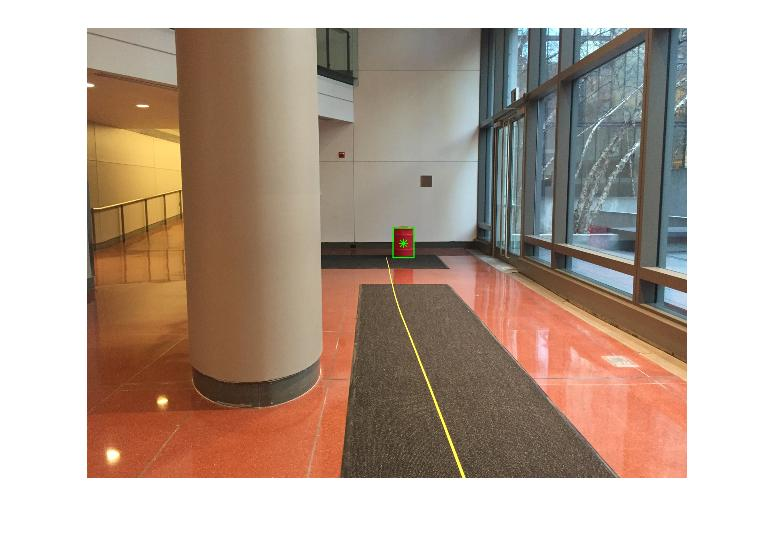
\includegraphics[trim={3cm 2cm 3cm 2cm},clip,scale=0.28]{results/006.jpg} & 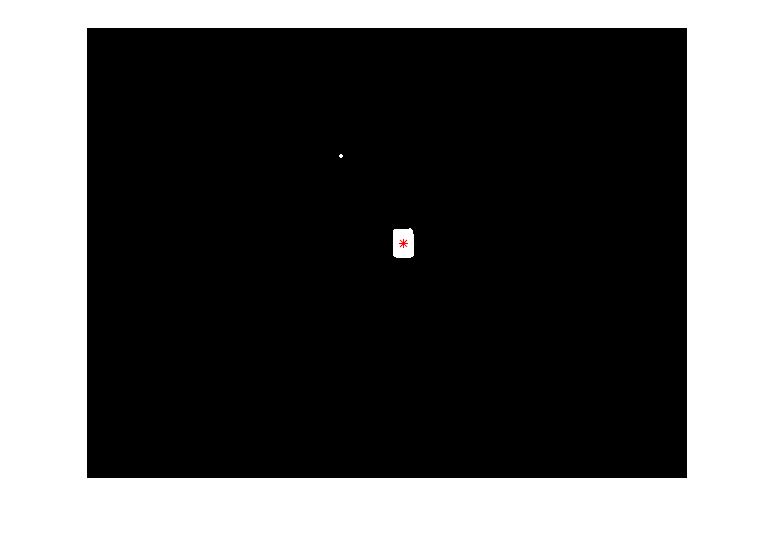
\includegraphics[trim={3cm 2cm 3cm 2cm},clip,scale=0.28]{results/006s.jpg} & \vspace{-4cm} x = 632.95, y = 430.65 & \vspace{-4cm}10.5322 \\ 
\hline 
\vspace{-4cm}007.png & 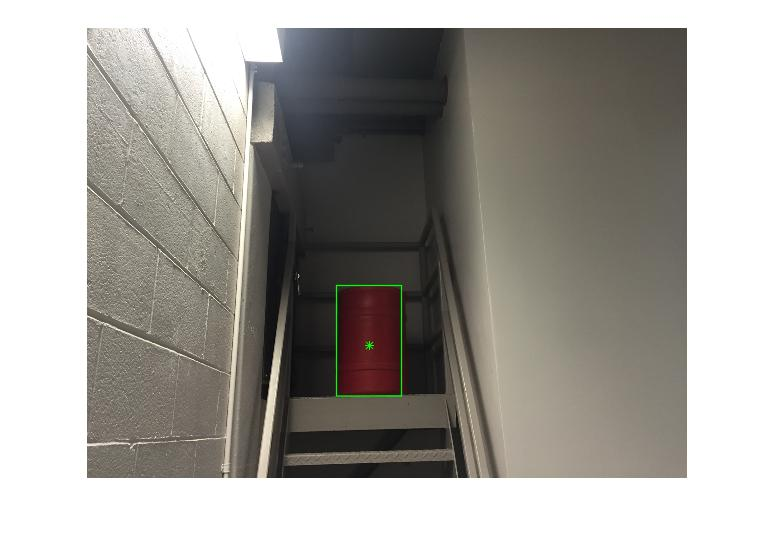
\includegraphics[trim={3cm 2cm 3cm 2cm},clip,scale=0.28]{results/007.jpg} & 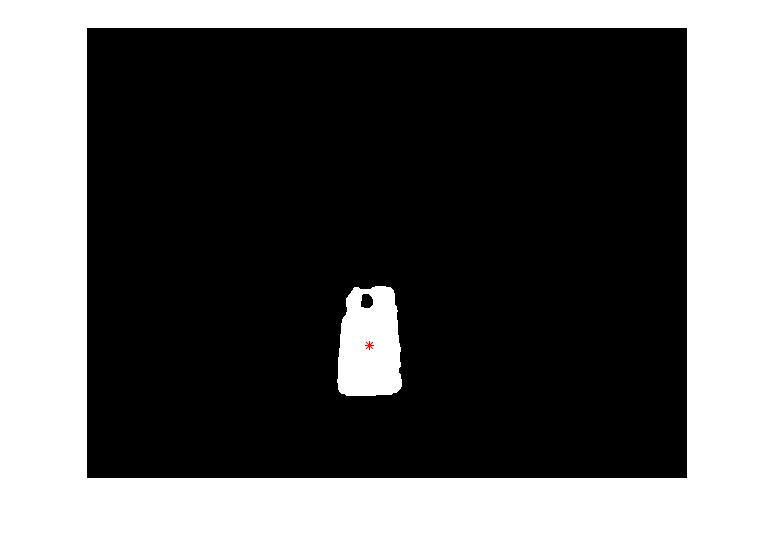
\includegraphics[trim={3cm 2cm 3cm 2cm},clip,scale=0.28]{results/007s.jpg} & \vspace{-4cm} x = 566.02, y = 634.66 & \vspace{-4cm}3.4350 \\ 
\hline 
\vspace{-4cm}008.png & 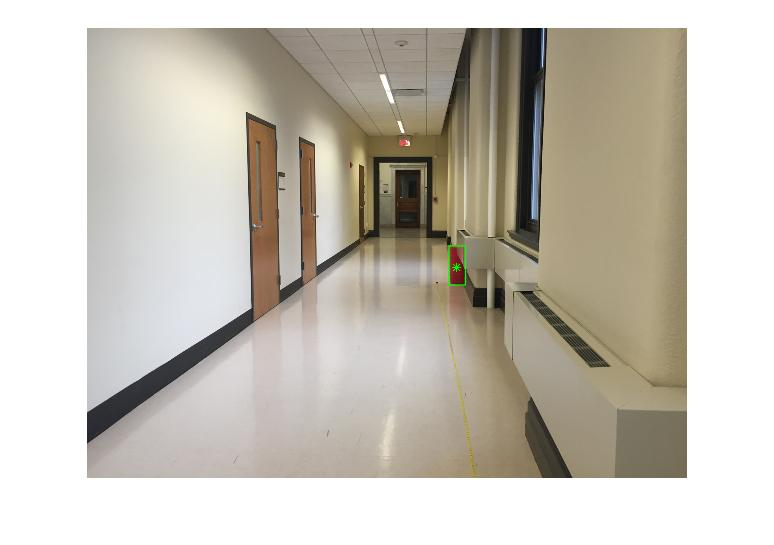
\includegraphics[trim={3cm 2cm 3cm 2cm},clip,scale=0.28]{results/008.jpg} & 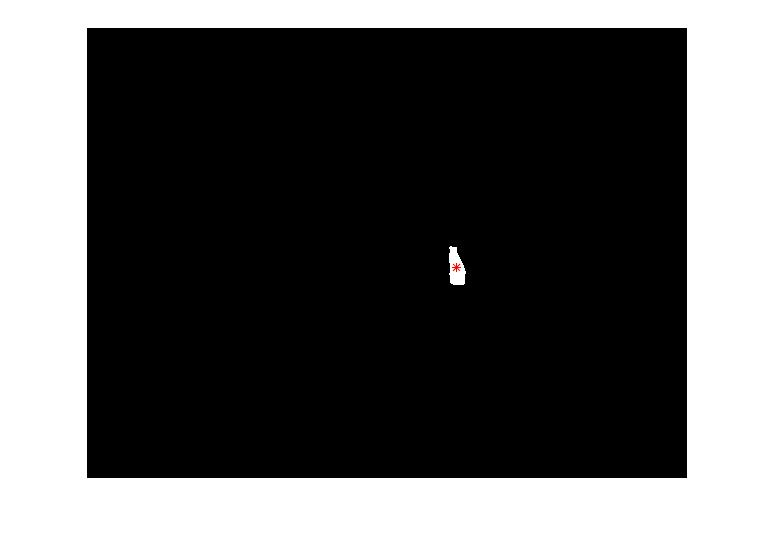
\includegraphics[trim={3cm 2cm 3cm 2cm},clip,scale=0.28]{results/008s.jpg} & \vspace{-4cm} x = 738.76, y = 480.19 & \vspace{-4cm}16.5787 \\ 
\hline 
\vspace{-4cm}009.png & 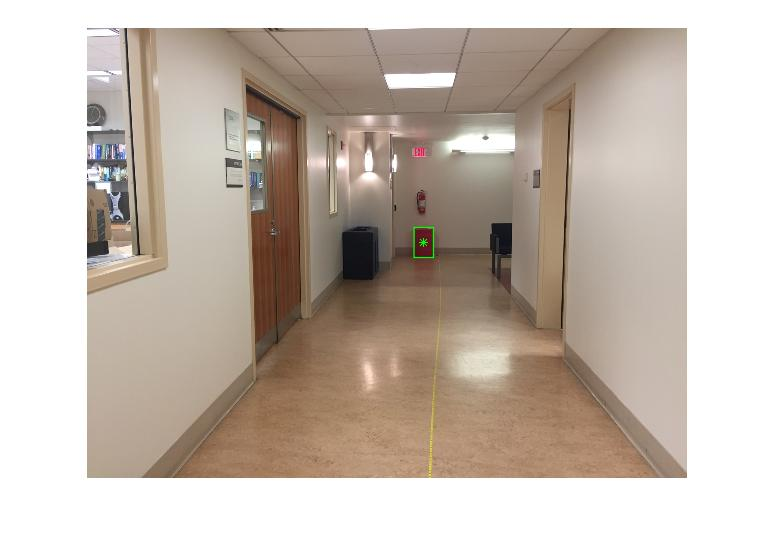
\includegraphics[trim={3cm 2cm 3cm 2cm},clip,scale=0.28]{results/009.jpg} & 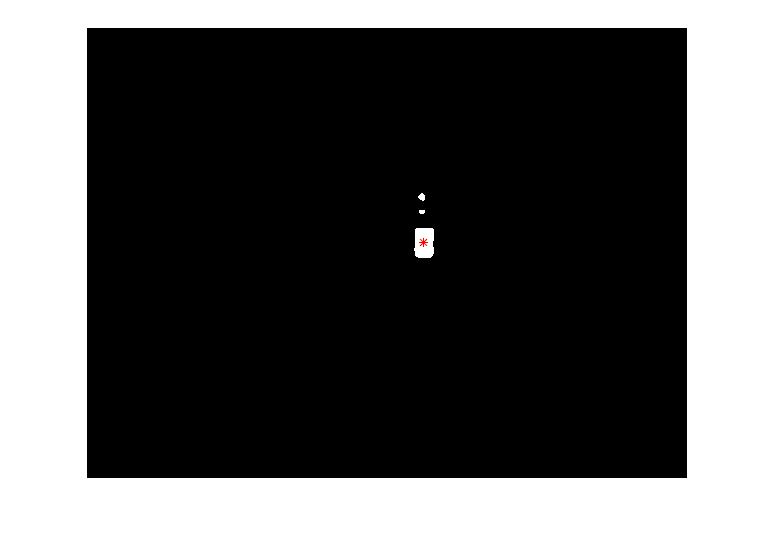
\includegraphics[trim={3cm 2cm 3cm 2cm},clip,scale=0.28]{results/009s.jpg} & \vspace{-4cm} x = 674.24, y = 429.40 & \vspace{-4cm}11.5428 \\ 
\hline 
\vspace{-4cm}010.png & 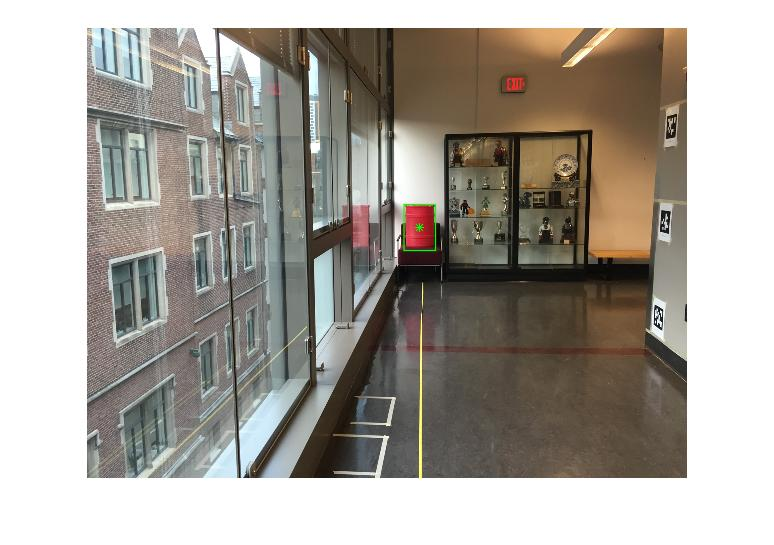
\includegraphics[trim={3cm 2cm 3cm 2cm},clip,scale=0.28]{results/010.jpg} & 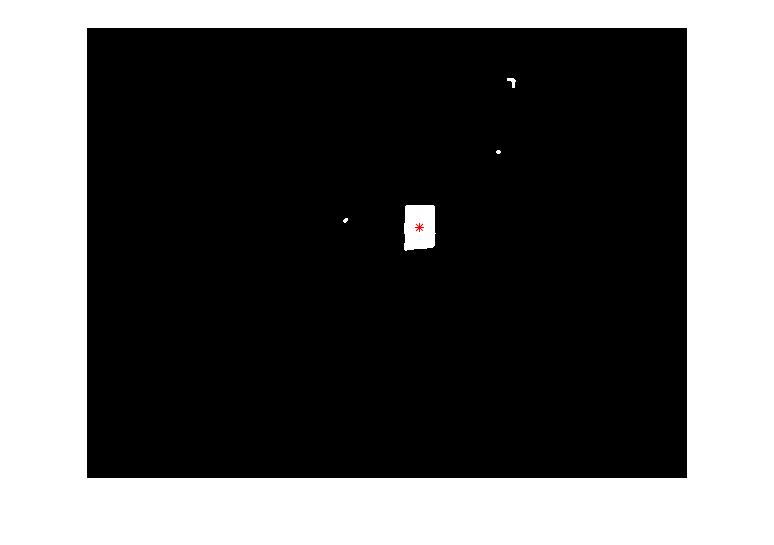
\includegraphics[trim={3cm 2cm 3cm 2cm},clip,scale=0.28]{results/010s.jpg} & \vspace{-4cm} x = 665.41, y = 398.55 & \vspace{-4cm}6.8694 \\ 
\hline 
\end{tabular} 
\end{table*}

\begin{thebibliography}{9}
\bibitem{Kraft} 
Kraft, Edgar. "A quaternion-based unscented Kalman filter for orientation tracking." Proceedings of the Sixth International Conference of Information Fusion. Vol. 1. 2003.
\end{thebibliography}

%----------------------------------------------------------------------------------------
%	REFERENCE LIST
%----------------------------------------------------------------------------------------
\phantomsection
\bibliographystyle{unsrt}
\bibliography{sample}

%---------------------------------------------------------------------------------------- 

\end{document}